\begin{frame}{Sparse Grids}{Requirements for a sparse grid}
    \begin{itemize}[<+->]
        \item A scalar valued function \(f\) which maps some input parameter \(\vb{x}\) to a scalar value \(f(\vb{x})\).
        \item \(f\) is defined on a unit hyper-cube \([0,1]^d\). Any input \(x_i\) should be transformed to \([0,1]\) easily.
        \item \(f\) can be computable in any point in hyper-cube.
        \item It is assumed that the function is \emph{computatinally expensive}. So that we need to change \(f\) with another function which is \emph{cheaper} and approximate original function well.
    \end{itemize}
\end{frame}

\begin{frame}{Sparse Grids}{Hierachical Basis Functions}
    \begin{columns}
        \begin{column}{0.5\textwidth}
            Using a standard hat function as a basis function, we can construct a sparse grid.

            \begin{equation*}
                \phi(x ) = \left\{
                \begin{array}{ll}
                    1-|x| & \text{if } x \in [-1,1] , \\
                    0     & \text{otherwise}          \\
                \end{array}
                \right.
                \label{eqn:basis}
            \end{equation*}
            \begin{figure}
                \centering
                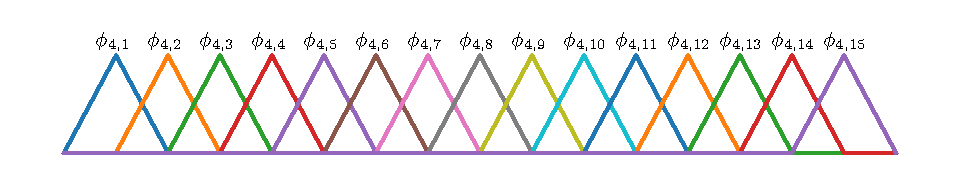
\includegraphics[width=\textwidth]{figures/nodal_basis.pdf}
                \caption{Nodal Basis Functions}
            \end{figure}
        \end{column}
        \begin{column}{0.5\textwidth}
            \begin{figure}
                \centering
                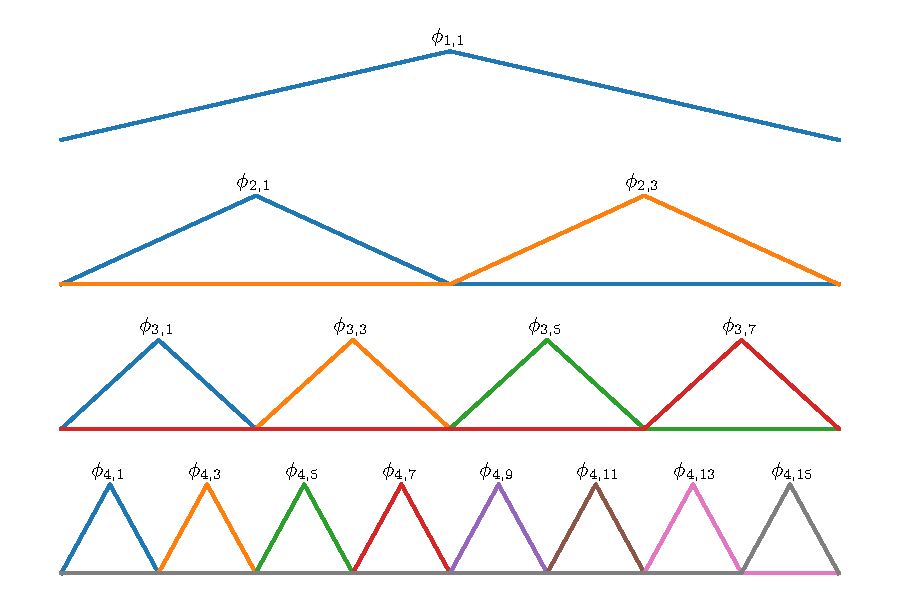
\includegraphics[width=\textwidth]{figures/hierarchical_basis.pdf}
                \caption{Hierarchical Basis Functions}
            \end{figure}
        \end{column}
    \end{columns}

\end{frame}

\begin{frame}{Sparse Grids}{Tensorial product and construction on d-dimensional space}
    \begin{figure}
        \centering
        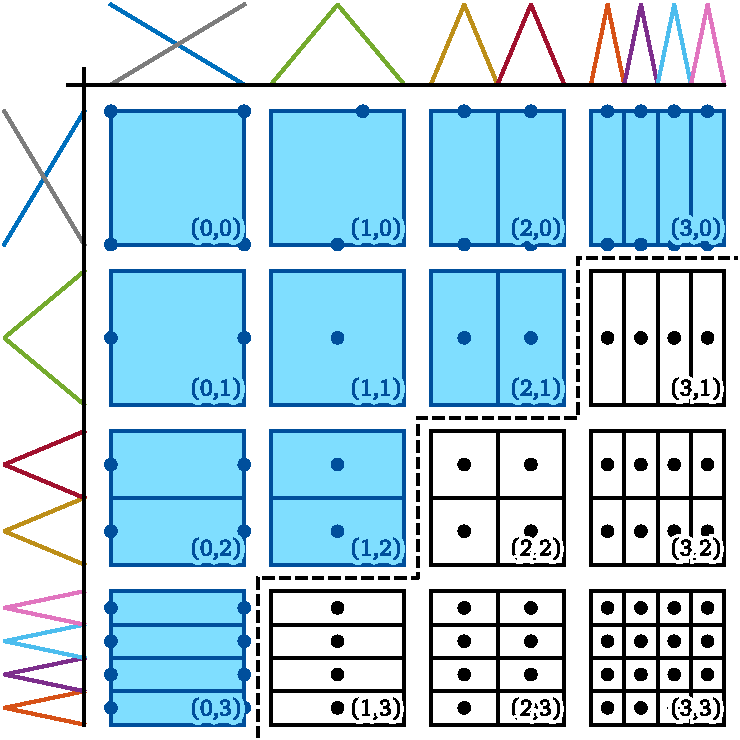
\includegraphics[width=\textwidth,height=0.6\textheight,keepaspectratio]{figures/sg_construction.pdf}
        \caption{Construction of the regular sparse grid of level in 2D, by \emph{Julian Valentin}}
    \end{figure}
\end{frame}
